\documentclass{article}
\usepackage[margin=1in, letterpaper]{geometry}
\usepackage[utf8]{inputenc}
\usepackage[english]{babel}
\usepackage{graphicx}
\usepackage[hidelinks]{hyperref}
\usepackage{enumitem}
\usepackage{amsmath}

\title{ECE324 Assignment 2}
\author{Frederick Boyd}
\date{September 19, 2019}

\begin{document}

\maketitle

\section{Solve by Inspection}
\begin{enumerate}[label=\roman*.]
  \item The answer we discussed in class is not unique. An example of another
        set of weights and biases that works is:
        \begin{equation*}
          \begin{bmatrix}
            w_0 & w_1 & w_2 \\
            w_3 & w_4 & w_5 \\
            w_6 & w_7 & w_8
          \end{bmatrix}
          =
          \begin{bmatrix}
            2  & -2 & 2  \\
            -2 & 2  & -2 \\
            2  & -2 & 2
          \end{bmatrix}
        \end{equation*}
        \begin{equation*}
          b = -8
        \end{equation*}
  \item $2^9 = 512$ unique inputs.
  \item Assuming we are always looking for an `x' that spans the entire grid,
        then the solution scales to a 4x4 and an NxN problem. This would work because
        the weights would just need follow a similar pattern. The weights where the `x'
        is expected to be would have a value of 1 and all other weights would be -1.
        The bias would scale similarly.
  \item No, because this would involve finding single-neuron parameters that
        have to activate the neuron in multiple scenarios. This complicates the problem
        significantly, making it difficult to find these parameters by hand.
\end{enumerate}

\section{Outputs to Hand In}
\subsection{Investigating Effect of Parameters on Accuracy}
\label{subsec:effect_of_parameters_on_accuracy}
The effect of the following parameters were investigated to see what effect
they have on the training and validation accuracy. Values of parameters other
than the one being investigated were kept constant. Those default values are:
\begin{itemize}
  \item Number of Epochs: 50
  \item Learning Rate: 0.2
  \item Activation Function: Linear
  \item Seed: 1
\end{itemize}

Effects of changing:
\begin{enumerate}
  \item \textbf{Number of Epochs:} See Table \ref{tab:epochs}.
        \begin{table}[ht]
          \label{tab:epochs}
          \begin{center}
            \caption{Effect of the number of epochs on training and validation accuracies.}
            \begin{tabular}{|c|c|c|}
              \hline
              \# of Epochs & Final Training Accuracy & Final Validation Accuracy \\ \hline
              5            & 0.795                   & 0.85                      \\ \hline
              10           & 0.95                    & 0.8                       \\ \hline
              25           & 0.975                   & 0.9                       \\ \hline
              50           & 0.975                   & 0.9                       \\ \hline
              75           & 0.98                    & 0.9                       \\ \hline
              100          & 0.98                    & 0.9                       \\ \hline
              500          & 0.98                    & 0.9                       \\ \hline
              1000         & 0.98                    & 0.9                       \\ \hline
            \end{tabular}
          \end{center}
        \end{table}

  \item \textbf{Learning Rate:} See Table \ref{tab:learning_rate}.
        \begin{table}[ht]
          \label{tab:learning_rate}
          \begin{center}
            \caption{Effect of the learning rate on training and validation accuracies.}
            \begin{tabular}{|c|c|c|}
              \hline
              Learning Rate & Final Training Accuracy & Final Validation Accuracy \\ \hline
              0.01          & 0.4                     & 0.25                      \\ \hline
              0.05          & 0.965                   & 0.85                      \\ \hline
              0.1           & 0.975                   & 0.9                       \\ \hline
              0.25          & 0.985                   & 0.9                       \\ \hline
              0.5           & 0.665                   & 0.35                      \\ \hline
              0.75          & 0.665                   & 0.35                      \\ \hline
              1             & 0.665                   & 0.35                      \\ \hline
            \end{tabular}
          \end{center}
        \end{table}

  \item \textbf{Activation Function:} See Table \ref{tab:act_function}.

        Using the default values in \ref{subsec:effect_of_parameters_on_accuracy}, it
        appears that ReLU is the best activation function. Compared to the linear and
        sigmoid activation functions, the ReLU function offers a good balance between
        the linear function's simplicity and the sigmoid's complexity.
        \begin{table}[ht]
          \label{tab:act_function}
          \begin{center}
            \caption{Effect of the activation function on training and validation accuracies.}
            \begin{tabular}{|c|c|c|}
              \hline
              Activation Function & Final Training Accuracy & Final Validation Accuracy \\ \hline
              Linear              & 0.975                   & 0.9                       \\ \hline
              ReLU                & 0.665                   & 0.65                      \\ \hline
              Sigmoid             & 0.98                    & 0.85                      \\ \hline
            \end{tabular}
          \end{center}
        \end{table}

  \item \textbf{Seed:} See Table \ref{tab:seed}.

        The training and validation
        accuracies differ slightly because the seed determines what random values the weights
        and bias initialize to. This, in turn, impacts the accuracies because the
        final weights and bias are directly determined from the random initial values.

        \textbf{NOTE:} When investigating the effect of various seeds on accuracy, the learning
        rate was kept constant at \textbf{0.25}, rather than the default value specified in
        section \ref{subsec:effect_of_parameters_on_accuracy}.
        \begin{table}[ht]
          \label{tab:seed}
          \begin{center}
            \caption{Effect of the activation function on training and validation accuracies.
              The learning rate for these values was kept constant at 0.25, rather than the
              default value specified in section \ref{subsec:effect_of_parameters_on_accuracy}.}
            \begin{tabular}{|c|c|c|}
              \hline
              Seed      & Final Training Accuracy & Final Validation Accuracy \\ \hline
              1         & 0.985                   & 0.9                       \\ \hline
              5         & 0.99                    & 0.9                       \\ \hline
              10        & 0.985                   & 0.9                       \\ \hline
              69        & 0.99                    & 0.85                      \\ \hline
              420       & 0.99                    & 0.85                      \\ \hline
              69 420    & 1.0                     & 0.85                      \\ \hline
              1 000 000 & 0.99                    & 0.85                      \\ \hline
            \end{tabular}
          \end{center}
        \end{table}
\end{enumerate}

\subsection{Best Parameters}
The following parameters generated the highest training and validation
accuracies. These values were determined empirically.
\begin{itemize}
  \item Learning Rate: 0.8
  \item Activation Function: Sigmoid
  \item Number of Epochs: 500
  \item Seed: 1
  \item Training Accuracy: 0.99
  \item Validation Accuracy: 1.0
\end{itemize}

Another set of parameters were empirically obtained that generate high
training and validation accuracies. However, these are rather extreme values.
More specifically, the learning rate is typically a value between 0 and 1,
which is not the case for the following set of values. This second set of parameters
is listed because while it achieves similar accuracies compared to the parameters
above in fewer epochs, it requires the use of extreme values which may not be
considered valid within the field of maching learning.
\begin{itemize}
  \item Learning Rate: 1000
  \item Activation Function: Sigmoid
  \item Number of Epochs: 5
  \item Seed: 1
  \item Training Accuracy: 0.99
  \item Validation Accuracy: 1.0
\end{itemize}

% \begin{figure}[ht]
%   \begin{center}
%     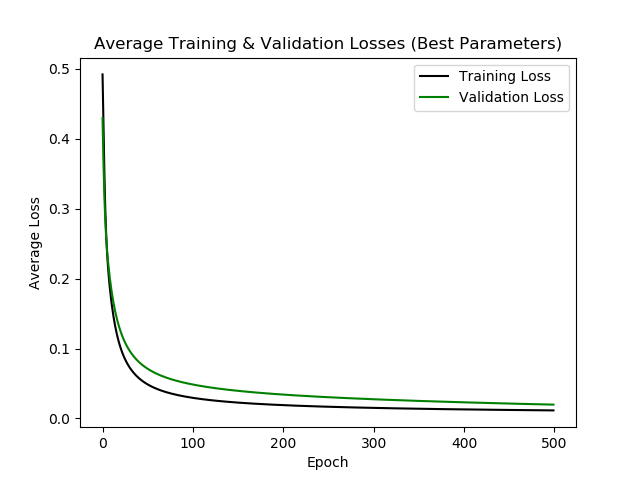
\includegraphics[width=0.7\linewidth]{figures/best-parameters-loss.png}
%     \caption{Average loss against the current epoch using the optimal parameters.}
%     \label{fig:best-parameters-loss}
%   \end{center}
% \end{figure}

% \begin{figure}[ht]
%   \begin{center}
%     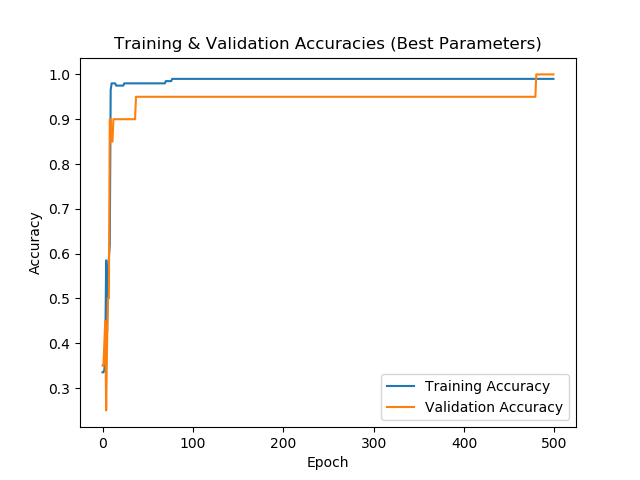
\includegraphics[width=0.7\linewidth]{figures/best-parameters-accuracies.png}
%     \caption{Training and validation accuracies against the current epoch using the 
%     optimal parameters.}
%     \label{fig:best-parameters-accuracies}
%   \end{center}
% \end{figure}

% \begin{figure}[ht]
%   \begin{center}
%     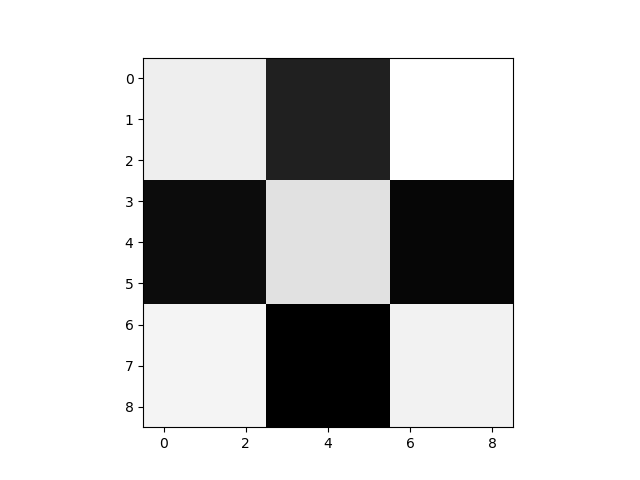
\includegraphics[width=0.7\linewidth]{figures/best-parameters-dispkernel.png}
%     \caption{Visualization of final weights using the best parameters using the 
%     \texttt{dispKernel} function.}
%     \label{fig:best-parameters-dispkernel}
%   \end{center}
% \end{figure}

\subsection{Written Questions}
\begin{enumerate}
  \item \textbf{Low Learning Rate}

        See Figures
        \ref{fig:low-rate-loss},
        \ref{fig:low-rate-accuracies}, and
        \ref{fig:low-rate-dispkernel} for plots of loss, accuracies, and
        a visualization of final weights, respectively. A learning rate of 0.01 was
        chosen. All other parameters were kept at their default values. The training
        and validation accuracies at the end of 50 epochs is significantly below 1.0,
        as seen in Figure \ref{fig:low-rate-accuracies}. Although the accuracy is
        gradually increasing during the last 20-30 epochs, it does so at a very slow
        rate. A similar issue can be seen with the plot of training and validation
        losses in Figure \ref{fig:low-rate-loss}. Although the average loss is
        decreasing, it does so at a rate that is not fast enough to reach
        approximately zero, even after 50 epochs. Since the learning rate is used to
        calculate the rate at which parameters should be adjusted, these issues are
        a result of the gradient descent calculations being scaled down too
        much. This, in turn, results in the single neuron not being able to minimize
        losses and achieve a reasonable accuracy within 50 epochs.
        \begin{figure}[ht]
          \begin{center}
            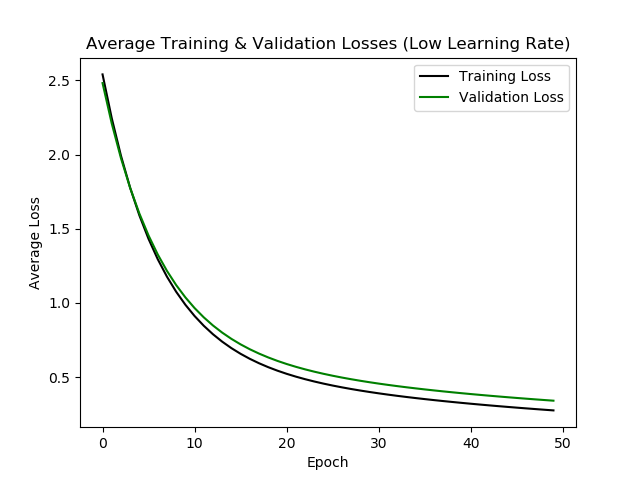
\includegraphics[width=0.7\linewidth]{figures/low-rate-loss.png}
            \caption{Average loss against the current epoch using a low learning rate.}
            \label{fig:low-rate-loss}
          \end{center}
        \end{figure}
        \begin{figure}[ht]
          \begin{center}
            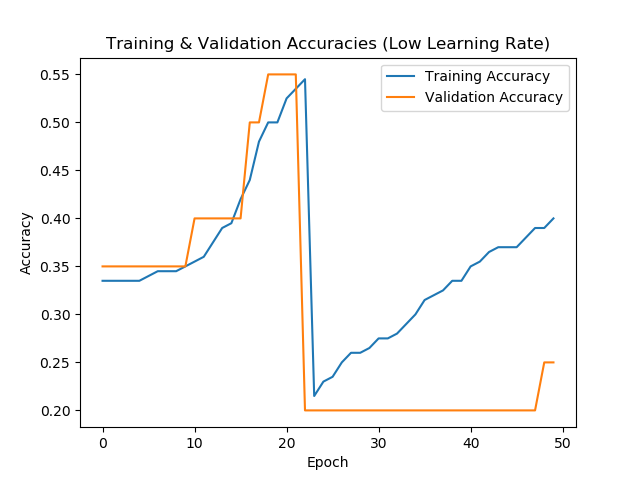
\includegraphics[width=0.7\linewidth]{figures/low-rate-accuracies.png}
            \caption{Training and validation accuracies against the current epoch using
              a low learning rate.}
            \label{fig:low-rate-accuracies}
          \end{center}
        \end{figure}
        \begin{figure}[ht]
          \begin{center}
            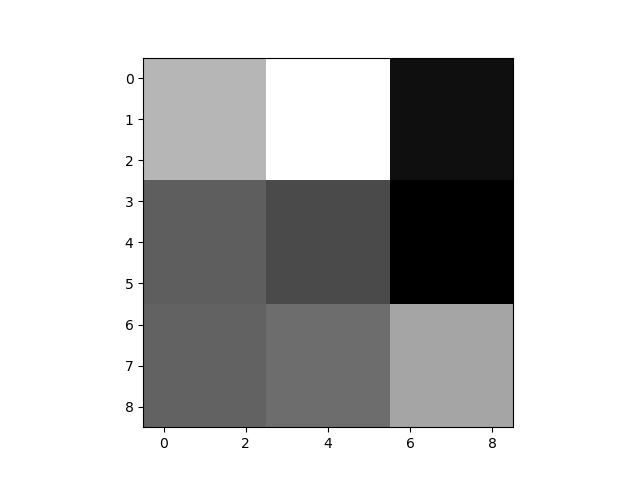
\includegraphics[width=0.7\linewidth]{figures/low-rate-dispkernel.png}
            \caption{Visualization of final weights with the \texttt{dispKernel}
              function using a low learning rate.}
            \label{fig:low-rate-dispkernel}
          \end{center}
        \end{figure}

  \item \textbf{High Learning Rate}

        See Figures \ref{fig:high-rate-loss},
        \ref{fig:high-rate-accuracies}, and
        \ref{fig:high-rate-dispkernel}
        for plots of loss, accuracies, and a visualization of
        final weights, respectively. A learning rate of 0.5 was chosen. All other
        parameters were kept at their default values. This learning rate resulted in
        exponentially increasing losses and oscillating accuracies. Although the
        visualization of weights using the \texttt{dispKernel} function looks good,
        a further investigation of the weights reveals that they are on the order of
        magnitude of $10^{22}$. The poor accuracies and ever-increasing losses are the
        result of the weights being adjusted too drastically, resulting in oscillations
        as the algorithm attempts to minimize losses. These oscillations can be seen
        in the training and validation accuracies in Figure
        \ref{fig:high-rate-accuracies}.
        \begin{figure}[ht]
          \begin{center}
            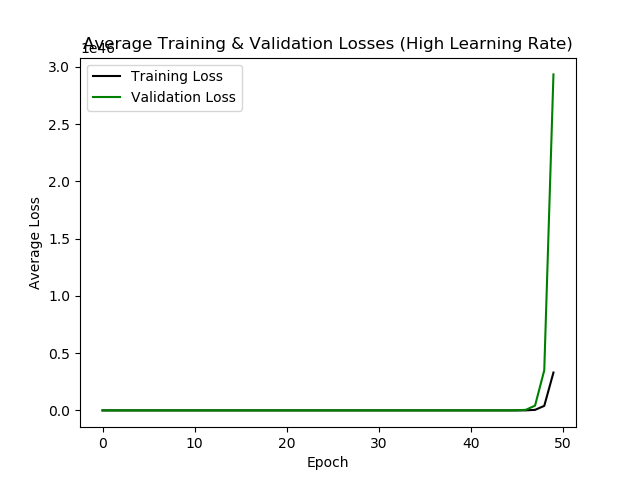
\includegraphics[width=0.7\linewidth]{figures/high-rate-loss.png}
            \caption{Average loss against the current epoch using a high learning rate.}
            \label{fig:high-rate-loss}
          \end{center}
        \end{figure}
        \begin{figure}[ht]
          \begin{center}
            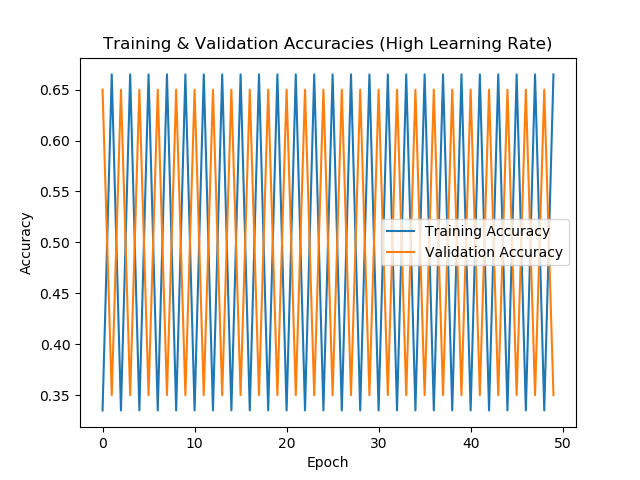
\includegraphics[width=0.7\linewidth]{figures/high-rate-accuracies.png}
            \caption{Training and validation accuracies against the current epoch using
              a high learning rate. The oscillations can be attributed to the algorithm
              adjusting weight values too drastically as it attempts to minimize losses.}
            \label{fig:high-rate-accuracies}
          \end{center}
        \end{figure}
        \begin{figure}[ht]
          \begin{center}
            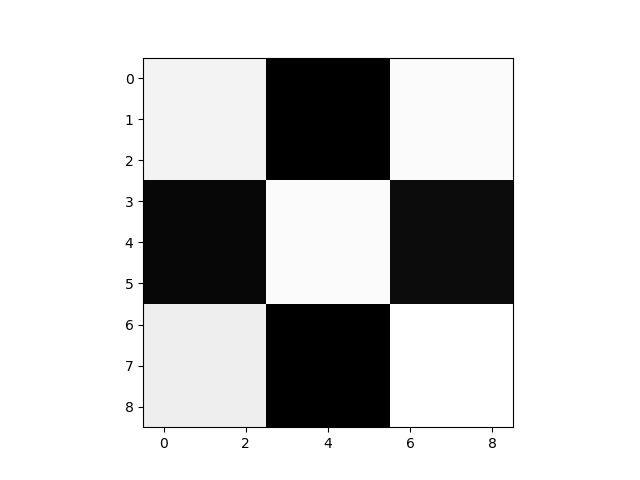
\includegraphics[width=0.7\linewidth]{figures/high-rate-dispkernel.png}
            \caption{Visualization of the final weights with the \texttt{dispKernel}
              function using a high learning rate. The final weights are on the order
              of magnitude of $10^{22}$.}
            \label{fig:high-rate-dispkernel}
          \end{center}
        \end{figure}

  \item \textbf{Good Learning Rate}

        See Figures \ref{fig:good-rate-loss},
        \ref{fig:good-rate-accuracies}, and
        \ref{fig:good-rate-dispkernel} for plots of loss, accuracies, and a
        visualization of final weights, respectively. A learning rate of 0.15 was
        chosen. All other parameters were kept at their default values.
        \begin{figure}[ht]
          \begin{center}
            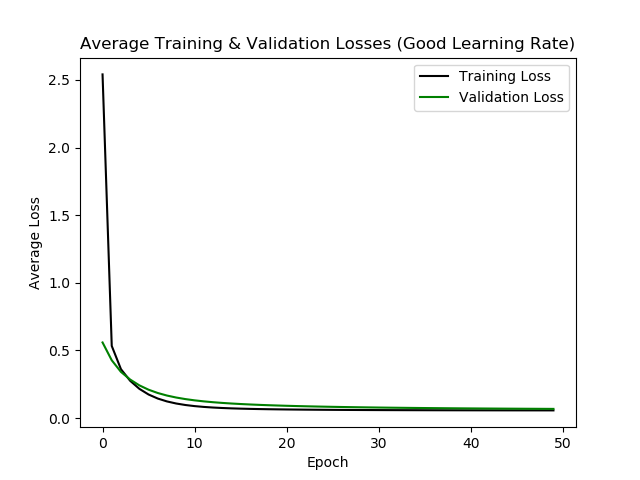
\includegraphics[width=0.7\linewidth]{figures/good-rate-loss.png}
            \caption{Average loss against the current epoch using a good learning rate.}
            \label{fig:good-rate-loss}
          \end{center}
        \end{figure}
        \begin{figure}[ht]
          \begin{center}
            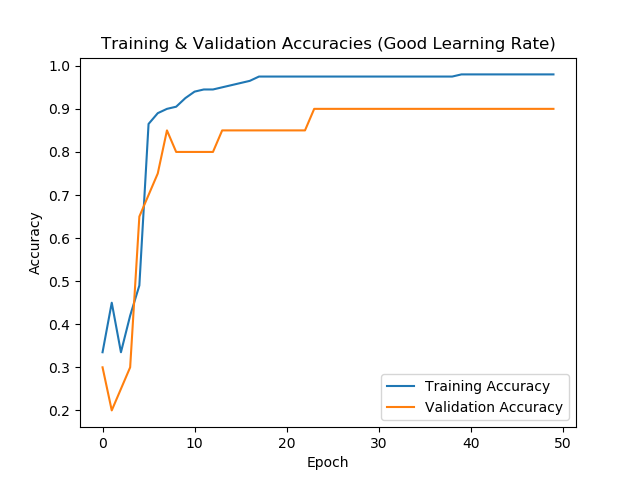
\includegraphics[width=0.7\linewidth]{figures/good-rate-accuracies.png}
            \caption{Training and validation accuracies against the current epoch using
              a good learning rate.}
            \label{fig:good-rate-accuracies}
          \end{center}
        \end{figure}
        \begin{figure}[ht]
          \begin{center}
            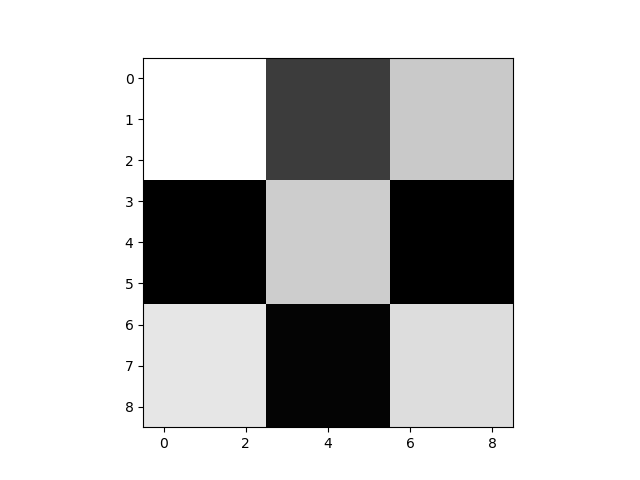
\includegraphics[width=0.7\linewidth]{figures/good-rate-dispkernel.png}
            \caption{Visualization of the final weights with the \texttt{dispKernel}
              function using a good larning rate.}
            \label{fig:good-rate-dispkernel}
          \end{center}
        \end{figure}

  \item \textbf{Plots for Three Activation Functions}

        Plots comparing the linear, ReLU, and sigmoid activation functions. Parameters
        were kept at their defaults except for the number of epochs, which was
        increased to 100.
        \begin{enumerate}
          \item \textbf{Linear Activation Function}

                See Figures \ref{fig:linear-loss},
                \ref{fig:linear-accuracies}, and
                \ref{fig:linear-dispkernel}
                for plots of loss, accuracies, and a visualization of final weights,
                respectively.
                \begin{figure}[ht]
                  \begin{center}
                    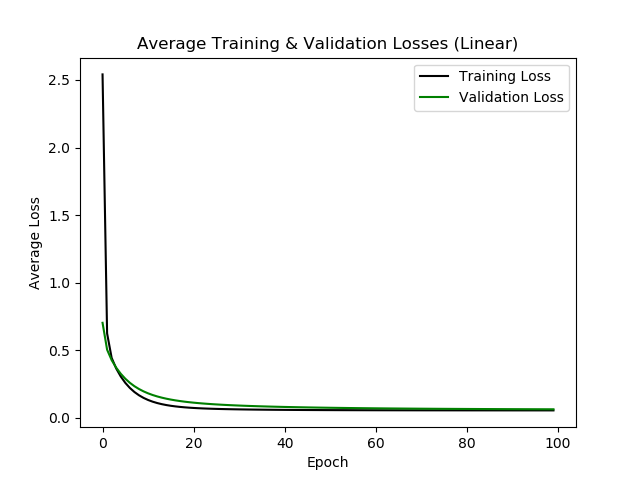
\includegraphics[width=0.7\linewidth]{figures/linear-loss.png}
                    \caption{Average loss against the current epoch using the linear
                      activation function.}
                    \label{fig:linear-loss}
                  \end{center}
                \end{figure}
                \begin{figure}[ht]
                  \begin{center}
                    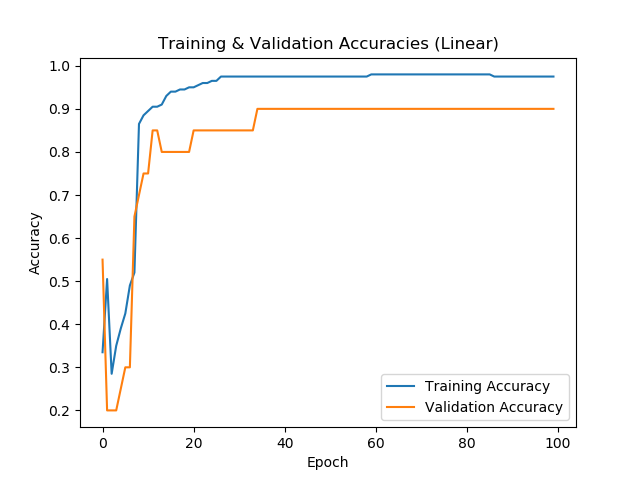
\includegraphics[width=0.7\linewidth]{figures/linear-accuracies.png}
                    \caption{Training and validation accuracies against the current epoch
                      using the linear activation function.}
                    \label{fig:linear-accuracies}
                  \end{center}
                \end{figure}
                \begin{figure}[ht]
                  \begin{center}
                    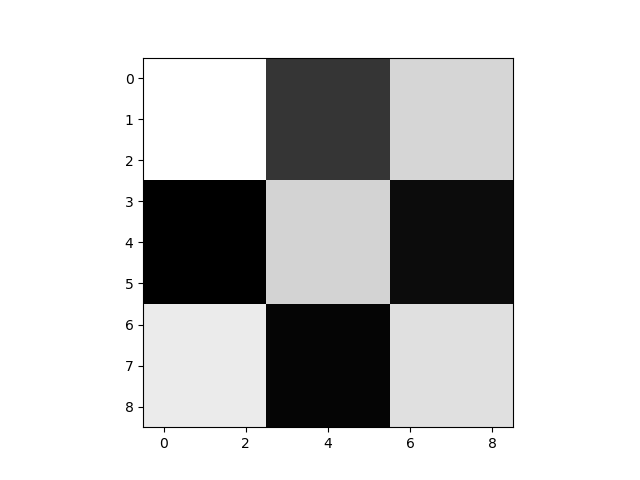
\includegraphics[width=0.7\linewidth]{figures/linear-dispkernel.png}
                    \caption{Visualization of final weights with the \texttt{dispKernel}
                      function using the linear activation function.}
                    \label{fig:linear-dispkernel}
                  \end{center}
                \end{figure}

          \item \textbf{ReLU Activation Function}

                See Figures \ref{fig:relu-loss},
                \ref{fig:relu-accuracies}, and
                \ref{fig:relu-dispkernel}
                for plots of loss, accuracies, and a visualization of final weights,
                respectively.
                \begin{figure}[ht]
                  \begin{center}
                    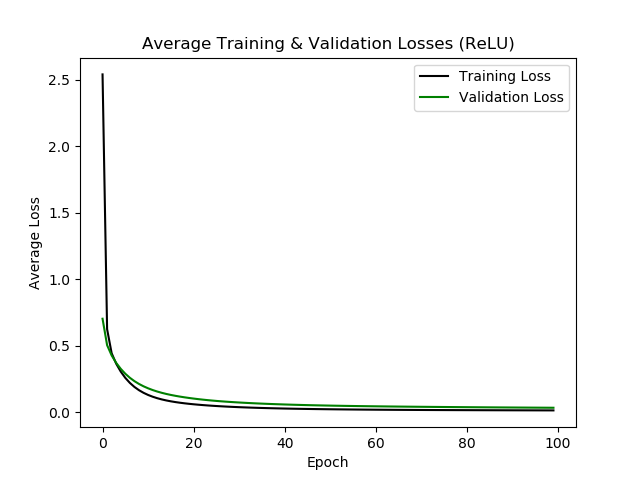
\includegraphics[width=0.7\linewidth]{figures/relu-loss.png}
                    \caption{Average loss against the current epoch using the ReLU
                      activation function.}
                    \label{fig:relu-loss}
                  \end{center}
                \end{figure}
                \begin{figure}[ht]
                  \begin{center}
                    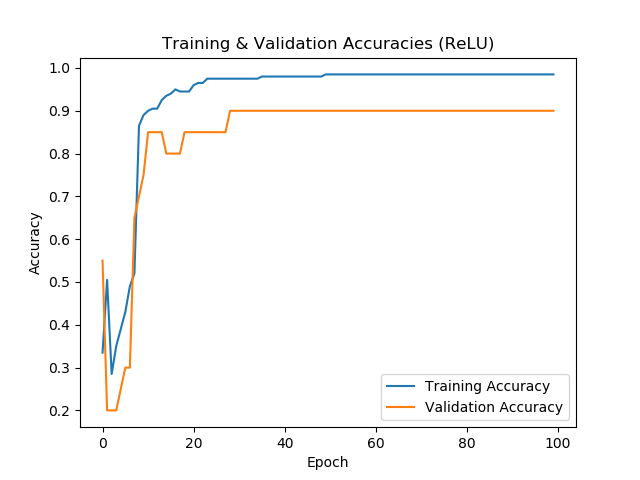
\includegraphics[width=0.7\linewidth]{figures/relu-accuracies.png}
                    \caption{Training and validation accuracies against the current epoch
                      using the ReLU activation function.}
                    \label{fig:relu-accuracies}
                  \end{center}
                \end{figure}
                \begin{figure}[ht]
                  \begin{center}
                    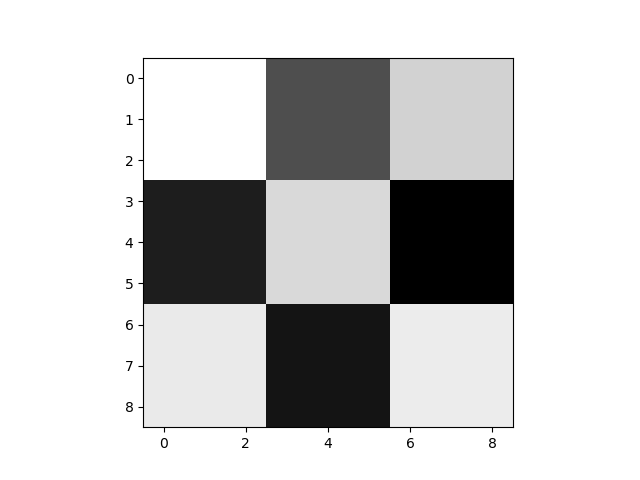
\includegraphics[width=0.7\linewidth]{figures/relu-dispkernel.png}
                    \caption{Visualization of the final weights with the \texttt{dispKernel}
                      function using the ReLU activation function.}
                    \label{fig:relu-dispkernel}
                  \end{center}
                \end{figure}

          \item \textbf{Sigmoid Activation Function}

                See Figures \ref{fig:sigmoid-loss},
                \ref{fig:sigmoid-accuracies}, and
                \ref{fig:sigmoid-dispkernel}
                for plots of loss, accuracies, and a visualization of final weights,
                respectively.
                \begin{figure}[ht]
                  \begin{center}
                    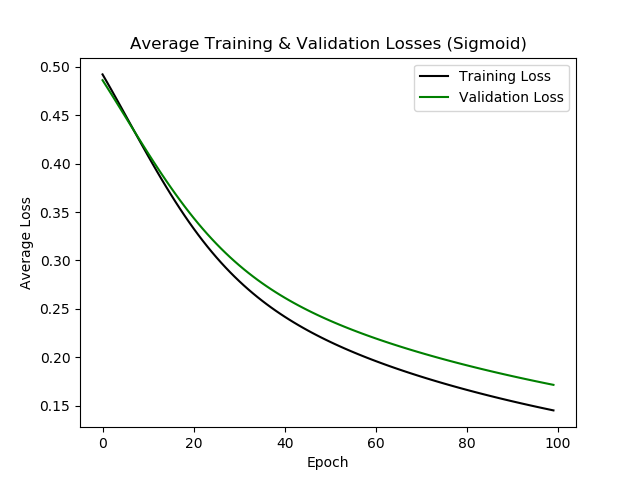
\includegraphics[width=0.7\linewidth]{figures/sigmoid-loss.png}
                    \caption{Average loss against the current epoch using the sigmoid
                      activation function.}
                    \label{fig:sigmoid-loss}
                  \end{center}
                \end{figure}
                \begin{figure}[ht]
                  \begin{center}
                    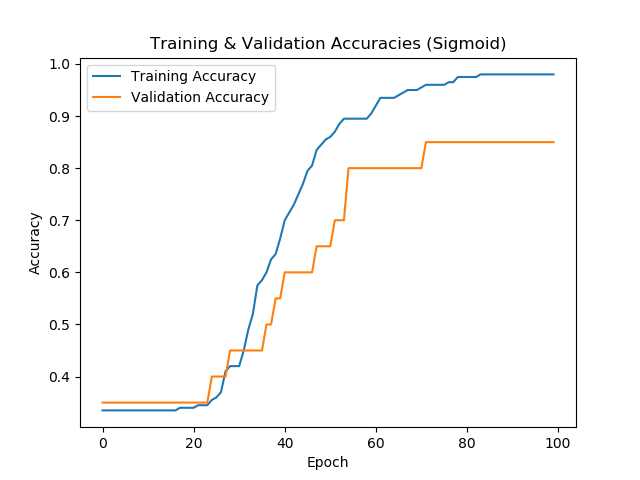
\includegraphics[width=0.7\linewidth]{figures/sigmoid-accuracies.png}
                    \caption{Training and validation accuracies against the current epoch
                      using the sigmoid activation function.}
                    \label{fig:sigmoid-accuracies}
                  \end{center}
                \end{figure}
                \begin{figure}[ht]
                  \begin{center}
                    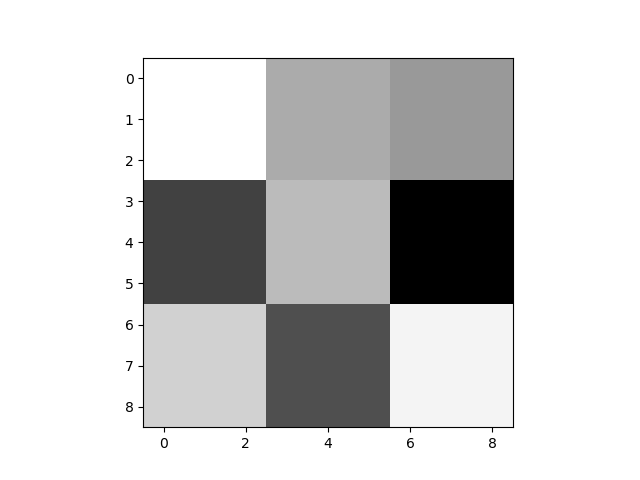
\includegraphics[width=0.7\linewidth]{figures/sigmoid-dispkernel.png}
                    \caption{Visualization of the final weights with the \texttt{dispKernel}
                      function using the sigmoid activation function.}
                    \label{fig:sigmoid-dispkernel}
                  \end{center}
                \end{figure}
        \end{enumerate}
\end{enumerate}

\end{document}
